\section{Background}
\label{section::background}

We begin with a brief overview of data center power provisioning infrastructure and power capping mechanisms.  A more extensive introduction to these topics is available in \cite{BarrosoBook09}.

\begin{figure*}[t]
\centering
\includegraphics[scale=.5]{Appendices/PowerRouting/figure/redundant.eps}
\vspace{-0.15 in}
\caption{ \textbf{Example power delivery system for a high-availability data center.} }
\vspace{-0.15 in}
\label{figure::redundant}
\end{figure*}


\textbf{Conventional power provisioning.} Today, most data centers operate according to power provisioning policies that assure sufficient capacity for every server. These policies are enforced by the data center operators at system installation time, by prohibiting deployment of any machine that creates the potential for overload.  Operators do their best to estimate systems' peak power draws, either through stress-testing, from vendor-supplied calculators, or through de-rating of nameplate specifications.

In high-availability data centers, power distribution schemes must also provision redundancy for fault tolerance; system deployments are further restricted by these redundancy requirements.  The Uptime Institute classifies data centers into tiers based on the nature and objectives of their infrastructure redundancy \cite{Turner05}. Some data centers provide no fault tolerance (Tier-1), or provision redundancy only within major power infrastructure components, such as the UPS system (Tier-2).  Such redundancy allows some maintenance of infrastructure components during operation, and protects against certain kinds of faults, but numerous single points-of-failure remain.  Higher-tier data centers provide redundant power delivery paths to each server. \PowerRouting is targeted at these data centers, as it exploits the redundant delivery paths to shift power delivery capacity.

\textbf{Example: A high-availability power system.} Figure~\ref{figure::redundant} illustrates an example of a high-availability power system design and layout for a data center with redundant distribution paths.  The design depicted here is based on the power architecture of the Michigan Academic Computer Center (MACC), the largest (10,000 square feet; 288 racks; 4MW peak load including physical infrastructure) of the three facilities providing utilization traces for this study. Utility power from two substations and a backup generator enter the facility at high voltage (13.2 kVAC) and meet at redundant automated transfer switches (ATS) that select among these power feeds.  These components are sized for the peak facility load (4MW), including all power infrastructure and cooling system losses.  The ATS outputs in turn are transformed to a medium voltage (480 VAC) and feed redundant uninterruptible power supply (UPS) systems, which are also each sized to support the entire facility.  These in turn provide redundant feeds to an array of power distribution units (PDUs) which further transform power to 208V 3-phase AC.  

PDUs are arranged throughout the data center such that each connects to two neighboring system clusters and each cluster receives redundant power feeds from its two neighboring PDUs.  The power assignments wrap from the last cluster to the first.  We refer to this PDU arrangement as a \emph{wrapped topology}. The wrapped topology provides redundant delivery paths with minimal wiring and requires each PDU to be sized to support  at most 150\% of the load of its connected clusters, with only a single excess PDU beyond the minimum required to support the load (called an ``N+1" configuration).  In the event of any PDU fault, 50\% of its supported load fails over to each of its two neighbors.  PDUs each support only a fraction of the data center's load, and can range in capacity from under ten to several hundred kilowatts.

Power is provided to individual servers through connectors (called ``whips"), that split the three phases of the 208VAC PDU output into the 120VAC single-phase circuits familiar from residential wiring.  (Some equipment may operate at higher voltages or according to other international power standards.) Many modern servers include redundant power supplies, and provide two power cords that can be plugged into whips from each PDU.  In such systems, the server internally switches or splits its load among its two power feeds.  For servers that provide only a single power cord, a rack-level transfer switch can connect the single cord to redundant feeds.

The capital costs of the power delivery infrastructure are concentrated at the large, high-voltage components: PDUs, UPSs, facility-level switches, generators, transformers and the utility feed.  The rack-level components cost a few thousand dollars per rack (on the order of \$1 per provisioned Watt), while the facility-level components can cost \$10-\$25 per provisioned Watt \cite{BarrosoBook09,Turner06}, especially in facilities with such high levels of redundancy.  With \PowerRouting, we focus on reducing the required provisioning of the facility-scale components while assuring a balanced load over the PDUs.  Though circuit breakers typically limit current both at the PDU's breaker panels and on the individual circuits in each whip, it is comparatively inexpensive to provision these statically to avoid overloads.  Though \PowerRouting is applicable to manage current limits on individual circuits, we focus on enforcing limits at the PDU level in this work.

\textbf{Phase balance}. In addition to enforcing current limits and redundancy, it is also desirable for a power provisioning scheme to balance power draw across the three phases of AC power supplied by each PDU.  Large phase imbalances can lead to current spikes on the neutral wire of a 3-phase power bus, voltage and current distortions on the individual phases, and generally increase heat dissipation and reduce equipment lifetime \cite{Gruzs90}.  Data center operators typically manually balance power draw across phases by using care in connecting equipment to particular receptacles wired to each phase.  \PowerRouting can automatically enforce phase balance by including it as explicit constraints in its scheduling algorithm. 


\textbf{Power capping.} Conservative, worst-case design invariably leads to power infrastructure over-provisioning \cite{Govindan09,Ranganathan06,Fan07,Wang09}.  Power capping mechanisms allow data center operators to sacrifice some performance in rare utilization spikes in exchange for substantial cost savings in the delivery infrastructure, without the risk of cascading failures due to an overload. In these schemes, some centralized control mechanism establishes a power budget for each server (e.g., based on historical predictions or observed load in the previous time epoch).  An actuation mechanism then enforces these budgets.  

\begin{figure*}[t]
\centering
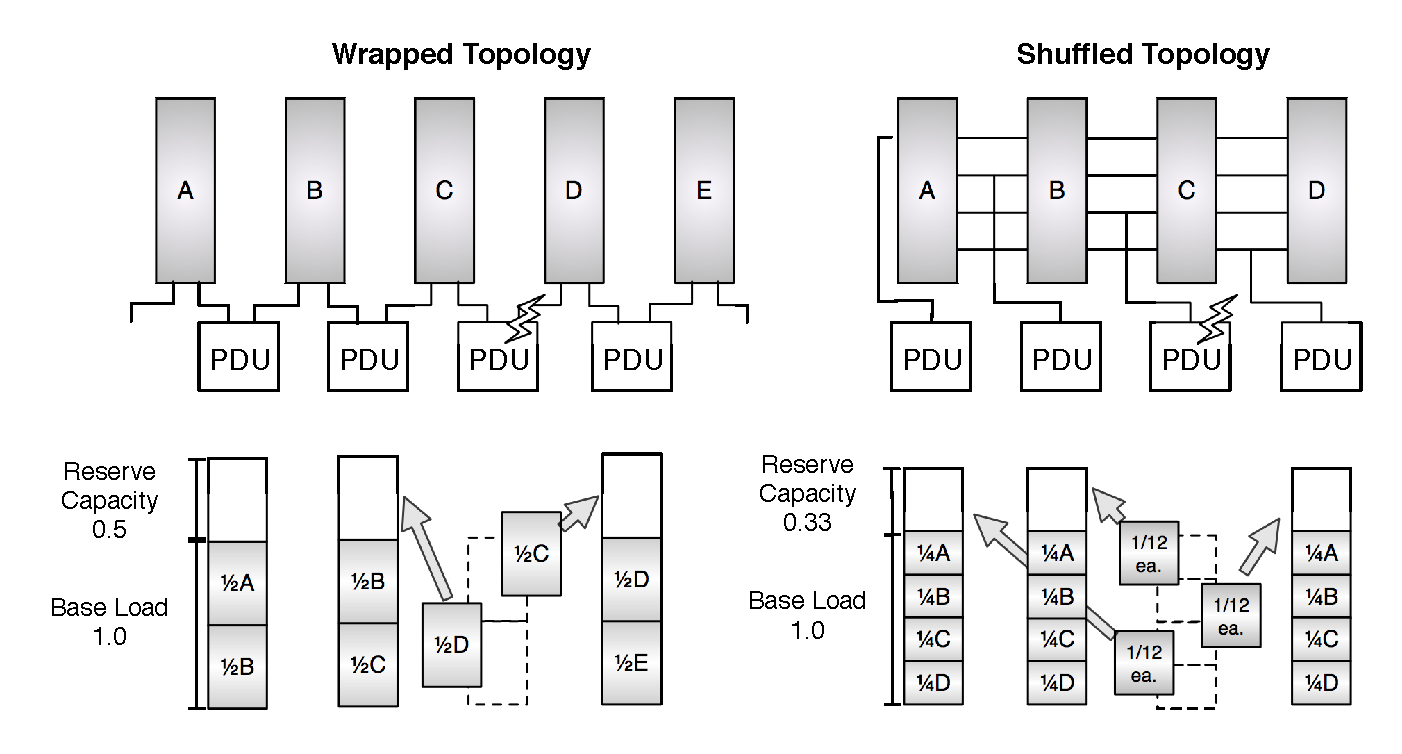
\includegraphics[width = 6.0 in]{Appendices/PowerRouting/figure/failover2.eps}
\caption{ \textbf{Reduced reserve capacity under shuffled topologies (4 PDUs, fully-connected topology).}}
\label{figure::failover}
\vspace{-.1 in}
\end{figure*}

The most common method of enforcing power budgets is through control loops that sense actual power draw and modulate processor frequency and voltage to remain within budget.  Commercial systems from IBM \cite{Popa06} and HP \cite{HP09} can enforce budgets to sub-watt granularities at milli-second timescales.  Researchers have extended these control mechanisms to enforce caps over multi-server chassis, larger ensembles, and entire clusters \cite{Ranganathan06,Lefurgy08,Wang08, Femal05}, examine optimal power allocation among heterogeneous servers \cite{Gandhi09b} and identify the control stability challenges when capping at multiple levels of the power distribution hierarchy \cite{Raghavendra08,Wang09}. Others have examined extending power management to virtualized environments \cite{Nathuji07}.  Soft fuses \cite{Govindan09} apply the notion of power budgets beyond the individual server and enforce sustained power budgets, which allow for transient overloads that the power infrastructure can support.  Finally, prior work considers alternative mechanisms for enforcing caps, such as modulating between active and sleep states \cite{Gandhi09a}. 

Like prior work, \PowerRouting relies on a power capping mechanism as a safety net to ensure extended overloads can not occur.  However, \PowerRouting is agnostic to how budgets are enforced. For simplicity, we assume capping based on dynamic frequency and voltage scaling, the dominant approach.  

Though rare, peak utilization spikes do occur in some facilities.  In particular, if a facility runs a single distributed workload balanced over all servers (e.g., as in a web search cluster), then the utilization of all servers will rise and fall together \cite{Fan07}.  No scheme that over-subscribes the physical infrastructure can avoid performance throttling for such systems. The business decision of whether throttling is acceptable in these rare circumstances is beyond the scope of this study; however, for any given physical infrastructure budget, \PowerRouting reduces performance throttling relative to existing capping schemes, by shifting loads among PDUs to locate and exploit spare capacity.

